	\PassOptionsToPackage{brazil,american}{babel}
\documentclass[12pt]{article}

\usepackage{sbc-template}
\usepackage[brazil,american]{babel}
\usepackage[utf8]{inputenc}

\usepackage{graphicx}
\usepackage{url}
\usepackage{float}
\usepackage{listings}	
\usepackage{color}
\usepackage{todonotes}
\usepackage{algorithmic}
\usepackage{algorithm}
\usepackage{hyperref}

\sloppy

\title{Experimento 10\\ 
	CONTADOR ASSÍNCRONO}

\author{
	Lucas Mafra Chagas, 12/0126443 \\
	Marcelo Giordano Martins Costa de Oliveira,  12/0037301
}


\address{Dep. Ciência da Computação -- Universidade de Brasília (UnB)\\
	CiC 116351 - Circuistos Digitais - Turma C
	\email{\{giordano.marcelo, chagas.lucas.mafra\}@gmail.com}
}

\begin{document}
	
	\maketitle
	
	\begin{abstract}
		In this experiment, we will develop a 4-stage progressive binary asynchronous counter using JK flip-flops.
	\end{abstract}
	
	\begin{resumo} 
		Nesse experimento, iremos desenvolver um contador assíncrono binário progressivo de 4 estágios utilizando flip-flops JK.
	
	\end{resumo}
	
	\section{Objetivos}
	\label{sec:Objetivos}
		Montar um contador assíncrono binário progressivo de 4 estágios, com flip-flops
		JK.Verificar a ocorrência de estados transitórios. Comparar com o funcionamento de
		um contador síncrono em anel. Projetar e montar um contador assíncrono binário
		reversível de 4 estágios, com flip-flops JK.
	
	
	\section{Materiais} 
	\label{sec:Materiais}
	
	\begin{itemize}
		\item software Quartus-II
		\item Kit de desenvolvimento DE2 com FPGA Altera Cyclone II.
	\end{itemize}
	
	\section{Introdução}
	\label{sec:Introducao}
	Contadores assíncronos variam de estado a cada pulso de um relógio, indo do seu valor atual para o seu valor consecutivo. Porém, como diz o nome, o contador assíncrono não tem todos os seus flip-flop envolvidos comandados pelo mesmo sinal de entrada do relógio. O primeiro flip-flop recebe um pulso e os outros estágios mudam de acordo com a saída do estágio anterior.  Por consequência, os estágios desse tipo de contador não se alteram simultaneamente, diferentemente do que ocorre com um contador síncrono. 
	Os contadores assíncronos são fáceis de se implementar, porém, eles são limitados, pois, como os estágios não são comandados pelo mesmo sinal de relógio, existe um certo atraso para cada estágio. Isso limita a velocidade de operação do contador, pois o pulso terá que ter um período mínimo para que todos os estágios tenham tempo de se alterar corretamente. 
	Esse atraso também causa estados transitórios no contador, que existem enquanto cada flip-flop não se estabelecem em uma nova situação. Portanto, temos que tomar cuidado ao conectar circuitos às saídas desse contador, pois se o circuito que interpreta essa saída for suficientemente rápido, ele poderá receber esses estados transitórios e como consequência, gerar resultados errados.  


	\section{Procedimentos}
	\label{sec:Procedimentos}
	

	
	\subsection{Contador Binário Progressivo Assícrono.}
	\label{2.1}
		Resolução das questões.
	
	\subsection{Implementação de um Contador Binário Progressivo Assíncrono.}
	\label{2.2}
	
	Para esta parte do experimento visava-se analisar o funcionamento de contador binário progressivo assíncrono e observar a presença de estados transitórios neste mesmo contador. O esquema do contador que seria construído encontra-se na figura abaixo:
	
	\begin{figure}[H]
		\centering
		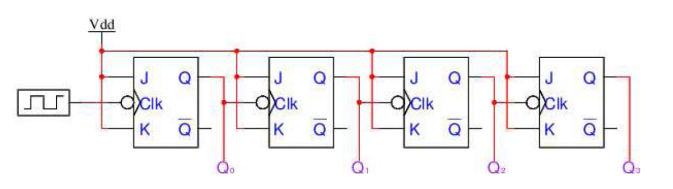
\includegraphics[width=1\textwidth]{contadorassincrono.png}
		\caption{Esquema de um contador binário progressivo assíncrono}
		\label{fig:contadorassincrono}
	\end{figure}
	
	Temos, porém, que além da estrutura apresentada na Figura A foi necessário adicionar uma porta NOR ao circuito, justamente para que o estado transitório 0000 fosse detectado. Portanto temos que as saídas Q0, Q1, Q2 e Q3 foram também utilizadas como entrada para essa porta NOR. Além disso, as saídas também foram conectadas a um decodificador para que o valor presente no contador aparecesse em um display de 7 segmentos.

	
	\subsection{Implementação de um Contador Anel.}
	\label{2.3}
	
	Nesta parte do experimento foi feita a implementação e análise de um contador em anel.
	
	

	\subsection{Implementação de um Contador Binário Reversível.}
	\label{2.4}
	
	a) Projetar e montar um contador binário reversível de 4 estágios, com flip-flops JK. O sentido de contagem deve ser dado por um terminal de controle (SC). A contagem será progressiva se SC = 1 e regressiva se SC = 0.
	
	O esquema criado para este contador encontra-se na imagem abaixo:
	
	\begin{figure}[H]
		\centering
		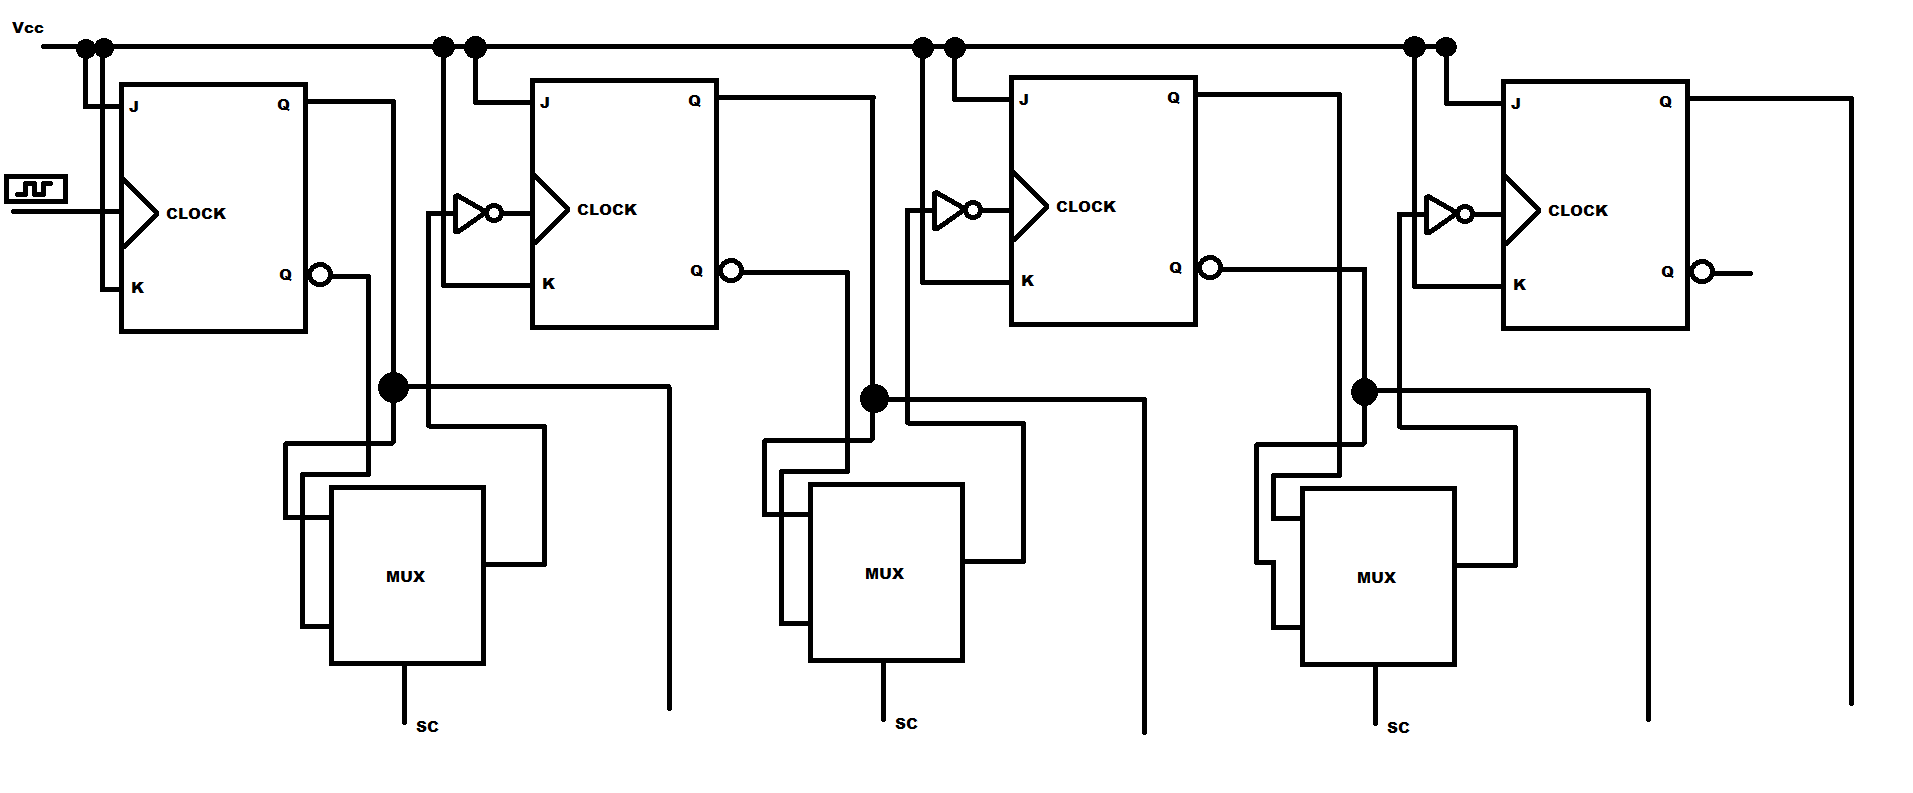
\includegraphics[width=1\textwidth]{contadorreversivel.png}
		\caption{Esquema de um contador binário progressivo assíncrono}
		\label{fig:Esquema de um contador binário reversível}
	\end{figure}
	
	Temos que se o Clock for igual a $\bar{Q}$ nós teremos um contador regressivo. Portanto, se queremos um contador que faz contagens regressivas e progressivas de acordo com a entrada SC, o único que precisamos fazer é definir qual entrada irá para o Clock do próximo flip-flop: Q ou $\bar{Q}$. Porém, sabemos que o circuito que escolhe uma de várias entradas é o multiplexador. Portanto, colocando SC como a entrada seletora, temos que se essa entrada for igual a 1 a saída será Q, caso contrário, ela será $\bar{Q}$. 
	
	b) Adicionar um segundo terminal de controle ao contador para evitar o problema de falso gatilho que pode ser causado durante uma transição de SC. O novo terminal (IC) deverá funcionar como um inibidor de contagem. Enquanto IC = 0, nenhum estágio deverá mudar de estado, independentemente do que ocorrer com Clk ou SC. Quando IC = 1, a contagem deverá ocorrer normalmente.
	
	
	Olhando a Figura B, vemos que todas as entradas J e K estão estabelecidas em 1, para que sempre que haja um pulso de relógio as saídas se inverterem gerando o efeito do contador. Porém, se estabelecermos ambas estas saídas em 0, teremos que cada flip-flop armazenará o último estado inserido, independente do Clock e da entrada SC. Portanto, para criar o inibidor de contagem IC, a única coisa que precisamos fazer é conectar todas as entradas J e K  a IC ao invés de conectá-las à Vcc. Quando IC = 1 a contagem ocorerrá normalmente como ocorria no caso da Figura B. Quando IC = 0 teremos a armazenagem do último estado e o contador permanecerá inerte.
	
	c)  Testar o funcionamento deste contador.   
	
	
	\section{Análise dos Resultados}
	\label{sec:Resultados}
	
	\subsection{Contador Binário Progressivo Assícrono.}
		\begin{flushleft}
			a) Qual é a máxima frequência do relógio para contagem confiável, no caso de 4 estágios?
		\end{flushleft}
		De acordo com o enunciado, temos que o período de cada flip-flop é entre 20ns e 25ns. Isso implica que o período do Clock deve ser maior do que a soma de todos esses períodos.
		
		Portanto, ficamos com:


		Trelogio $ > $ N $*$ 20/25 como temos 4 flip-flops, então N$=$4.

		Trelogio $>$ 80ns$/$100ns

		Logo, temos que a frequência do Clock será o inverso do período, ou seja:
	
		
		frelogio $>$ 12,5MHz/10MHz 
		
		
	\begin{flushleft}
		b)	Suponha que o relógio tenha uma frequencia de 18MHz Qual será o maior número de estágios que podem ser decodificados sem erros por um circuito combinacional nas saídas do contador.
	\end{flushleft}

		
		Fazendo o processo oposto da questão anterior para descobrir N:
		
		
		frelogio $=$ 18MHz $=$ 18000000 Hz
		
		frelogio $=$ 18000000 Hz $=$ 1/T
		
		frelogio $=$ 18000000 Hz $=$ 1/T
		
		T $=$ 0,000000055 $=$ 55ns
		
		55ns $=$ N $*$ 20/25
		
		N $=$ 2,75/2,20
		
		
		Poderemos ter então, no máximo, 2 flip-flops.
		
	\begin{flushleft}
		c)	Suponha que o relógio tenha uma frequência de 10 Hz e uma porta NOR de 4 entradas seja
		usada para decodificar o estado 0000. Em que transições da sequência de contagem (0 a 15)
		esse estado será identificado na forma de uma flutuação transitória na saída da porta?
	\end{flushleft} 
	
	Observando a tabela abaixo é possível identificar os pontos em que temos o estado 0000.
	
	\begin{table}[H]
		\centering
		\begin{tabular}{|c|c|c|c|c|}
			\cline{1-5}
			\multicolumn{1}{|c|}{Nº de pulsos} & \multicolumn{4}{|c|}{Sequencia de Contagem} \\
			\hline
			 & Q0 & Q1 & Q2 & Q3 \\
			\hline
			0  & 0 & 0 & 0 & 0 \\
			\hline
			1  & 1 & 0 & 0 & 0 \\
			\hline
			2  & 0 & 1 & 0 & 0 \\
			\hline
			3  & 1 & 1 & 0 & 0 \\
			\hline
			4  & 0 & 0 & 1 & 0 \\
			\hline
			5  & 1 & 0 & 1 & 0 \\
			\hline
			6  & 0 & 1 & 1 & 0 \\
			\hline
			7  & 1 & 1 & 1 & 0 \\
			\hline
			8  & 0 & 0 & 0 & 1 \\
			\hline
			9  & 1 & 0 & 0 & 1 \\
			\hline
			10  & 0 & 1 & 0 & 1 \\
			\hline
			11  & 1 & 1 & 0 & 1 \\
			\hline
			12  & 0 & 0 & 1 & 1 \\
			\hline
			13  & 1 & 0 & 1 & 1 \\
			\hline
			14  & 0 & 1 & 1 & 1 \\
			\hline
			15  & 1 & 1 & 1 & 1 \\
			\hline
		\end{tabular}
	\end{table}

	Vemos que para qualquer transição de em que temos Q0 indo de 0 para 1 não teremos esse problema. Isso acontece devido ao fato de que Q0 será a primeira saída a ser alterada quando acontecer uma mudança de estado. Portanto, se essa saída está indo de 0 para 1 teremos que o resultado final será 1XXX onde X é um valor que não importa já que aqui queremos apenas identificar os estados onde teremos a transitório 0000.
	Consequentemente, temos que:
	
	\begin{itemize}
		\item Quando vamos do pulso 1 para o pulso 2,  temos 1000 indo para 0100. Quando a saída  Q0 sofrer a alteração ( e ela sofrerá essa alteração antes das outras) temos que o estado será momentaneamente 0000. Ele mudará apenas quando Q1 receber o sinal de mudança.
		\item Quando vamos do pulso 3 para o pulso 4, temos 1100 indo para 0010. Temos que quando Q0 se altera ficamos com o estado intermediário 0100. Depois, quando Q1 se altera ficamos com outro estágio intermediário 0000. Portanto, haverá a sinalização na porta NOR. Esse estado se encerrará quando Q2 receber o pulso e alterar o seu valor.
		\item Finalmente, quando vamos do pulso 7 para o pulso 8, temos 1110 indo para 0001. Quando Q0 se alterar vamos para o estado intermediário 0110. Teremos um novo estágio intermediário 0010 quando Q1 se alterar. Então, quando Q2 sofrer a alteração ficaremos com 0000 até que Q3 se altere. 
	\end{itemize}

	
	\subsection{Implementação de um Contador Binário Progressivo Assíncrono.}
	
	\begin{figure}[H]
		\centering
		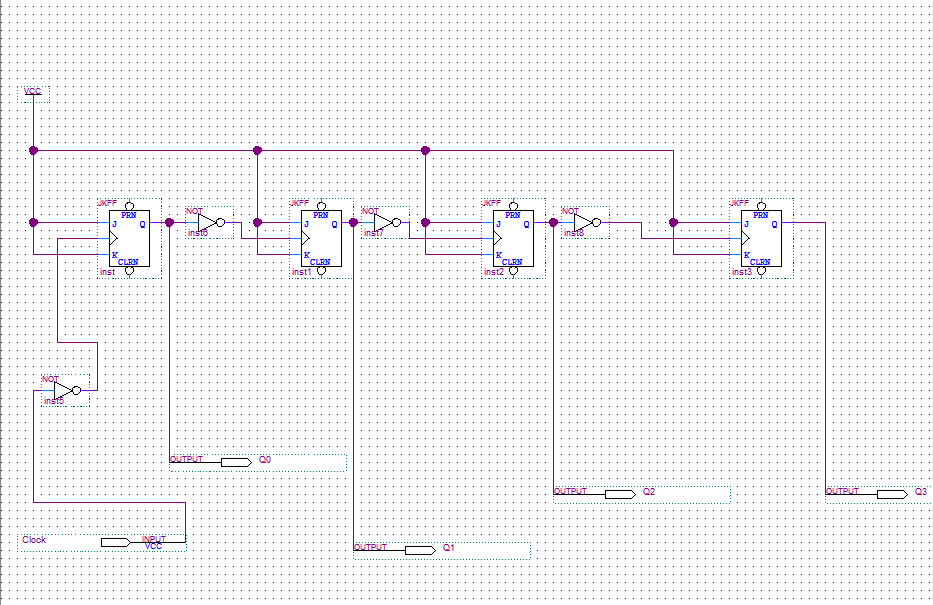
\includegraphics[width=1\textwidth]{contadorjk.png}
		\caption{Implementação do contador assíncrono com a utilização de flip-flops JK}
		\label{fig:contadorjk}
	\end{figure}
	
	Como o flip-flop disponível no programa possuía as entradas PRESET e CLEAR elas foram simplesmente ignoradas para não influenciar o resultado. Gerando a simulação real (que considera atrasos de propagação de portas) de tempo para esse circuito, obteve-se o seguinte diagrama em forma de onda:
	
	\begin{figure}[H]
		\centering
		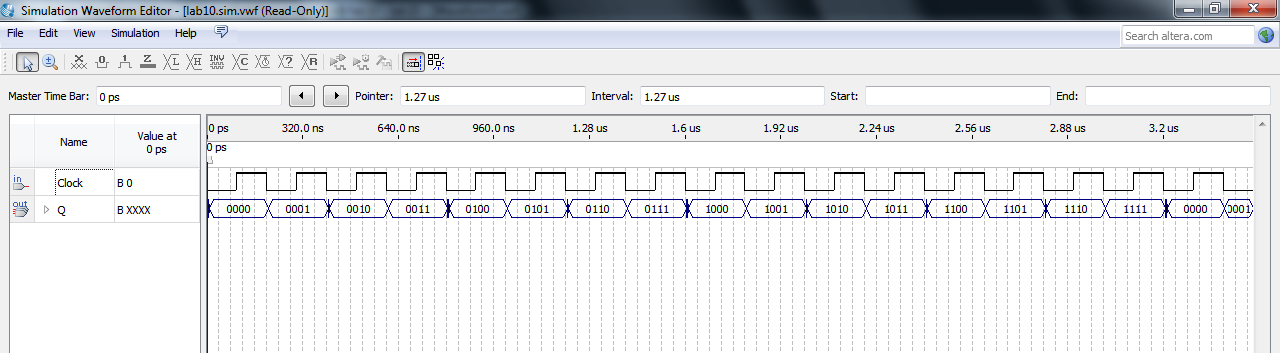
\includegraphics[width=1\textwidth]{contadorondas.png}
		\caption{Implementação do contador assíncrono com a utilização de flip-flops JK}
		\label{fig:contadorondas}
	\end{figure}
	
	Vemos neste diagrama que existem mudanças de estado que são seguidas por linhas azuis marcantes.Ampliando o diagrama foi possível perceber que essas linhas nada mais são do que os estados transitórios, ocorrendo rapidamente, tornando-se quase invisíveis no diagrama quando ele não está ampliado.Fez-se o registro de todos os estados transitórios e a partir disso foi possível gerar a seguinte tabela:
	
		\begin{table}[H]
			\centering
			\begin{tabular}{|c|c|}
				\cline{1-2}
				\multicolumn{1}{|c|}{Transição} & \multicolumn{1}{|c|}{Estado Transitório}\\
				\hline
				0000 $\rightarrow $ 0001  & X \\
				\hline
				0001 $\rightarrow $ 0010  & 0000  \\
				\hline
				0010 $\rightarrow $ 0011  & X \\
				\hline
				0011 $\rightarrow $ 0100  & 0010 0000  \\
				\hline
				0100 $\rightarrow $ 0101  & X \\
				\hline
				0101 $\rightarrow $ 0110  & 0100  \\
				\hline
				0110 $\rightarrow $ 0111  & X \\
				\hline
				0111 $\rightarrow $ 1000  & 0110 0100 0000  \\
				\hline
				1000 $\rightarrow $ 1001  & X \\
				\hline
				1001 $\rightarrow $ 1010  & 1000  \\
				\hline
				1010 $\rightarrow $ 1011  & X \\
				\hline
				1011 $\rightarrow $ 1100  & 1010 1000  \\
				\hline
				1100 $\rightarrow $ 1101  & X \\
				\hline
				1101 $\rightarrow $ 1110  & 1100  \\
				\hline
				1110 $\rightarrow $ 1111  & X \\
				\hline
				1111 $\rightarrow $ 0000  & 1110 1100 1000  \\
				\hline
			\end{tabular}
		\end{table}
	
	
	
	Vemos pela tabela que todas as transições de números pares para números ímpares não possuem estados transitórios. Isso se dá pelo fato de que a mudança de um número par para o seu consecutivo ímpar ocorre apenas no bit menos significativo, em nosso contador representado pela saída Q0. Q0 é o primeiro elemento do contador a sofrer a mudança após um pulso do Clock, e na transição de um número par para um número ímpar ele é o único que precisa sofrer essa mudança. Então, apesar de as outras saídas sofrerem com o atraso de propagação, elas não irão se alterar após receberem o sinal, e, por isso, não temos estados transitórios para esses casos. 
	Além disso é possível verificar pela tabela que as previsões feitas para o estado transitório 0000 estavam corretas. Ele apareceu na transição de 0001 para 0010, na transição de 0011 para 0100 e na transição de 0111 para 1000. 
	Outras transições possuem outros valores para seus estados transitórios. Vemos que estes estados transitórios sempre possuem diferença de um bit entre si, sendo que o primeiro estado transitório apresenta diferença de um bit em relação ao valor atual do contador e o último apresenta um bit de diferença em relação ao próximo valor que será gerado pelo contador. Isso simplesmente evidencia a assincronicidade do contador e os atrasos de cada um dos 3 flip-flops. É possível concluir desse fato que teremos um número de estados transitórios igual ao número de bits diferentes entre os valores consecutivos menos 1. Menos 1 pois a transição do primeiro flip-flop (Q0) é sempre a que inicia a mudança dos outros, logo, não teremos atrasos referentes a este flip-flop. Um exemplo disso é a transição de 0111 para 1000. Vemos que nesta transição temos 3 estados transitórios. Os números 0111 e 1000 possuem 4 bits de diferença e 4 - 1 = 3. Além disso vemos que o primeiro estado transitório 0110 possui apenas um bit de diferença em relação à 0111 e o último estado transitório 0000 possui apenas um bit de diferença em relação à 1000.
	Depois da obtenção do diagrama de ondas para este circuito, inseriu-se um decodificador de display de 7 segmentos a ele, e cada saída foi conectada a uma entrada desse codificador. Além disso foi inserida uma porta NOR que recebia como entradas Q0, Q1, Q2 e Q3. Isso foi feito para a identificação do estado 4.
	Após programar a placa Altera para que ela gerasse resultados referentes a este circuito, foi observado o comportamento na placa. 
	
	
	
	Obviamente, não foi possível observar estados transitórios de 4 na placa, pois o período de duração desses estados era da ordem de nanosegundos, e, mesmo conectado à saída, o olho humano não consegue acompanhar a velocidade com que ele se acende e se apaga ao detectar um estado transitório.
	
	
	
	\subsection{Implementação de um Contador Anel.}
	
	\begin{figure}[H]
		\centering
		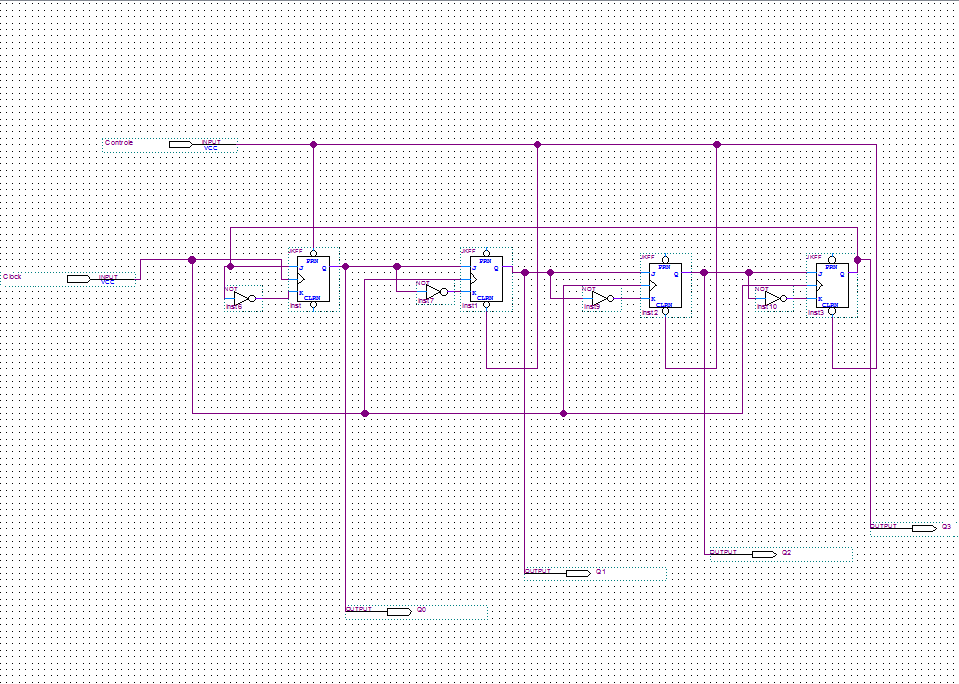
\includegraphics[width=1\textwidth]{contadoranel.png}
		\caption{ Implementação do contador em anel}
		\label{fig:contadoranel}
	\end{figure}
	
	
	
	Temos que as entradas de PRESET e CLEAR foram utilizadas para inicializar o contador. A entrada de CLEAR foi ativada no primeiro flip-flop enquanto a entrada de PRESET foi inicializada nas outras, fazendo o estado inicial do contador ser 1000 (com a ordem da saída dos flip-flops sendo Q0Q1Q2Q3). Feita a inicialização, depois disso o contador passou a agir como registrador. Além disso, como o contador em anel normalmente é criado a partir da utilização de flip-flops D, o flip-flop JK organizado de tal forma a representar esse flip-flop. A entrada K recebia o inverso da entrada J. Além disso, como o contador em anel é um circuito sequencial síncrono temos que todos os flip-flop recebem o mesmo sinal de Clock. A partir dessa implementação obteve-se o seguinte diagrama de ondas:
	
	\begin{figure}[H]
		\centering
		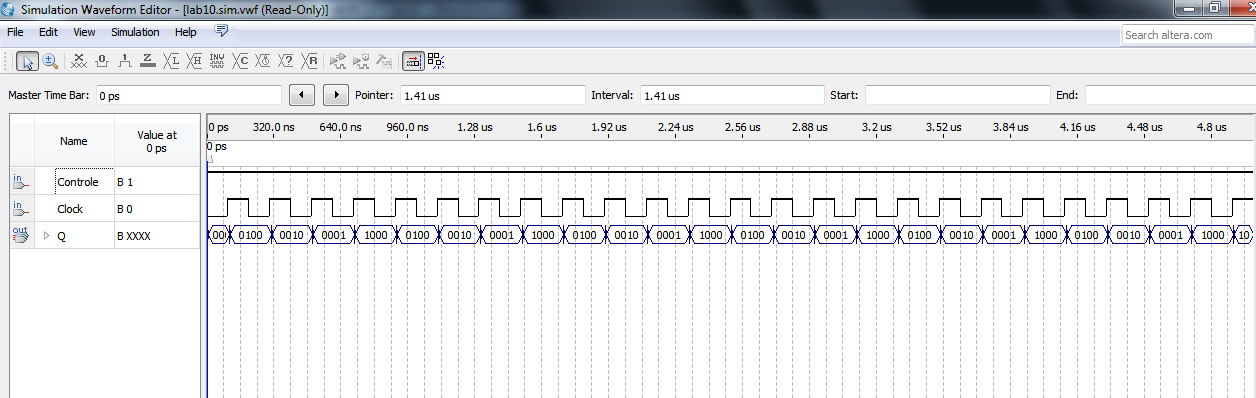
\includegraphics[width=1\textwidth]{contadoranelondas1.png}
		\caption{ Diagrama de ondas para o contador em anel}
		\label{fig:contadoranelondas1}
	\end{figure}
	
	Vemos que o contador seguiu o padrão esperado, agindo como um registrador. A cada passagem do relógio vemos que a posição do bit contendo o 1 se desloca uma posição para a direita. Como no caso anterior, temos que o contador possui estados transitórios. Ampliando a figura é possível evidenciar isso:
	
	\begin{figure}[H]
		\centering
		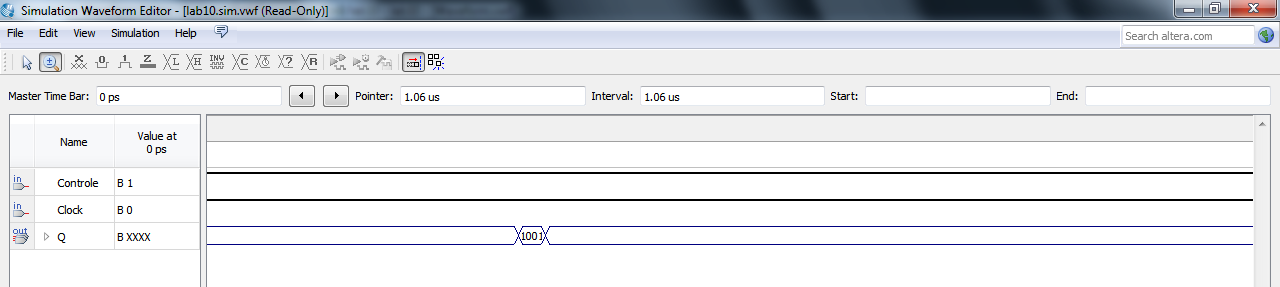
\includegraphics[width=1\textwidth]{contadoranelondas2.png}
		\caption{ Diagrama de ondas ampliado. O estado transitório apresentado nesta imagem é o estado 1001 obtido na transição de 0001 para 1000}
		\label{fig:contadoranelondas2}
	\end{figure}
	
	Visualizando os estados transitórios para os outros casos foi possível criar a seguinte tabela:
	
		\begin{table}[H]
			\centering
			\begin{tabular}{|c|c|}
				\cline{1-2}
				\multicolumn{1}{|c|}{Transição} & \multicolumn{1}{|c|}{Estado Transitório}\\
				\hline
				0001 $\rightarrow $ 0010  & 0000  \\
				\hline
				0010 $\rightarrow $ 0100  & 0000 \\
				\hline
				0100 $\rightarrow $ 1000  & 0000 \\
				\hline
				1000 $\rightarrow $ 0001  & 1001  \\
				\hline
			\end{tabular}
		\end{table}
	
	Vemos que para quase todos os casos o estado transitório obtido é 0000. Isso se dá pelo fato de que a transição sempre ocorre antes em Q0 indo em ordem crescente até Q3. De tal forma, temos que o próximo estado do contador, em todos os casos apresentará o 1 em uma posição Qi+1. Qi então se altera para 0 antes que Qi+1 o faça, gerando o estado 0000. O único caso em que isso não acontece é na transição de 1000 para 0001, pois temos que Q0 sofrer a mudança para 1 antes que Q3 volte a ser 0 (aqui a posição de 1 não se encontra em um Qi+1), gerando o estado transitório 1001. 
	
	

	\subsection{Implementação de um Contador Binário Reversível.}
	
	A partir do circuito projetado foi possível implementar o circuito do contador reversível. Porém, para facilitar a implementação e diminuir o número de circuitos muito complexos, o multiplexador que selecionava a entrada Q ou Q foi substituída por uma porta XOR. Essa implementação é preferível também devido ao fato de o flip-flop JK presente no programa Quartus não possuir a saída Q. Com uma porta XOR temos que toda vez que a entrada SC for 0 a saída será o próprio Q. Toda vez que a entrada SCfor 1 a saída será Q. Isso é evidenciado pela tabela abaixo:
	
	\begin{table}[H]
		\centering
		\begin{tabular}{|c|c|c|}
			\cline{1-3}
			\multicolumn{1}{|c|}{SC} & \multicolumn{1}{|c|}{Q} &
			\multicolumn{1}{|c|}{Saída}\\
			\hline
			0 & 0 & 0 \\
			\hline
			0 & 1 & 1 \\
			\hline
			0 & 0 & 1 \\
			\hline
			1 & 1 & 0 \\
			\hline
		\end{tabular}
	\end{table}
	
	
	Porém, ao adotar essa solução temos que o contador irá ter contagem progressiva quando SC = 0 ao invés de SC = 1. Poderíamos ter colocado uma porta NOT antes da entrada SC para evitar isso, porém, durante a implementação deixou-se o circuito com SC inverso.
	Além de SC temos que como o flip-flop do programa Quartus possui as entradas PRESET e CLEAR temos que ICpode ser implementado com a ajuda dessas portas ao invés de ser conectado às entradas J e K. Como temos que o flip-flop dará prioridade para PRESET e CLEAR, se estes estiverem conectados a 1 temos que o flip-flop não estará setado nem resetado e apenas armazenará o estado em que ele se encontrava antes de isso ocorrer. Portanto, o estado anterior será mantido, independente das entradas SC e Clock. Caso contrário, o contador irá funcionar normalmente. 
	Temos, então, de acordo com as mudanças detalhadas acima, que a implementação do flip-flop contador binário reversível ficou da seguinte forma:
	
	\begin{figure}[H]
		\centering
		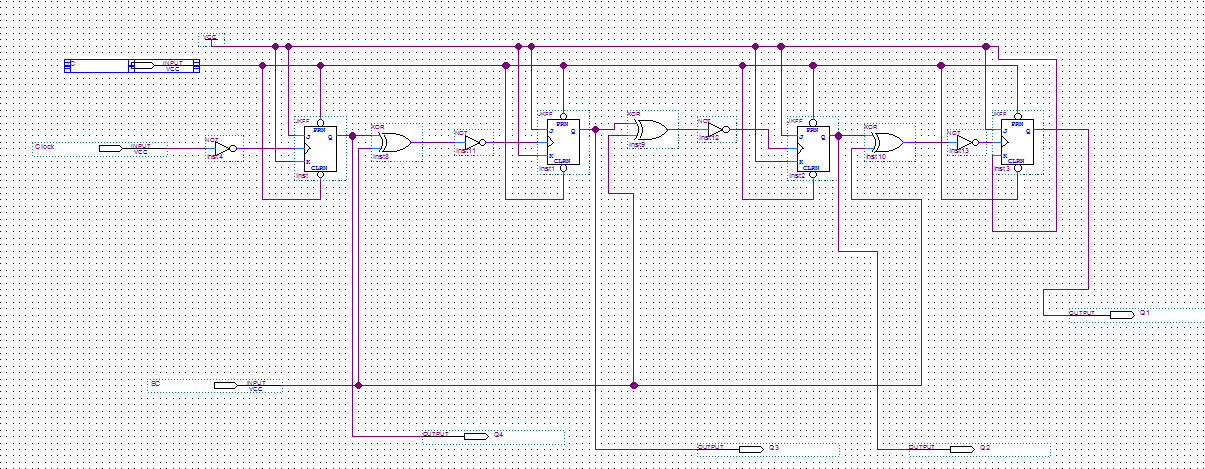
\includegraphics[width=1\textwidth]{contadorreversivel2.png}
		\caption{ Implementação do contador binário reversível Obs.: uma porta NOT foi depois adicionada neste esquema após a entrada IC para que o circuito se mantivesse estável quando IC=0 ao invés de quando IC=1 }
		\label{fig:contadorreversivel2}
	\end{figure}
	
	Para este contador obteve-se as seguintes formas de onda: 

	\begin{figure}[H]
		\centering
		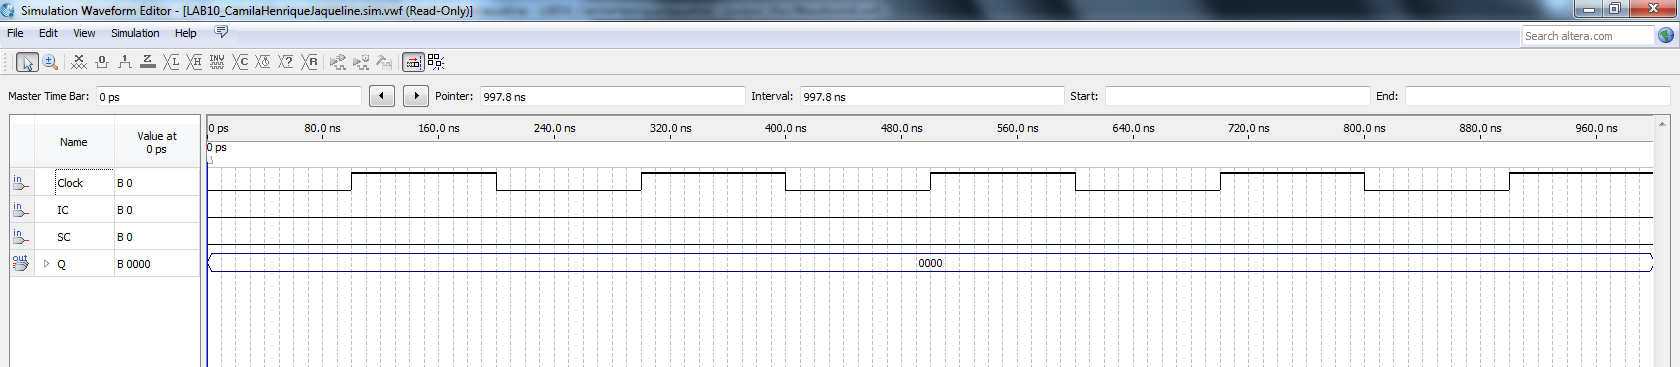
\includegraphics[width=1\textwidth]{contadorreversivelonda1.png}
		\caption{ Onda obtida quando a entrada IC se encontrava em 0 }
		\label{fig:contadorreversivelonda1}
	\end{figure}
	
	Vemos aqui que o contador segue o padrão esperado: IC está desativado e portanto não há contagem, apenas armazenamento do último estado do contador. Obs.: para o diagrama de ondas dessa parte do experimento, 
	

	\begin{figure}[H]
		\centering
		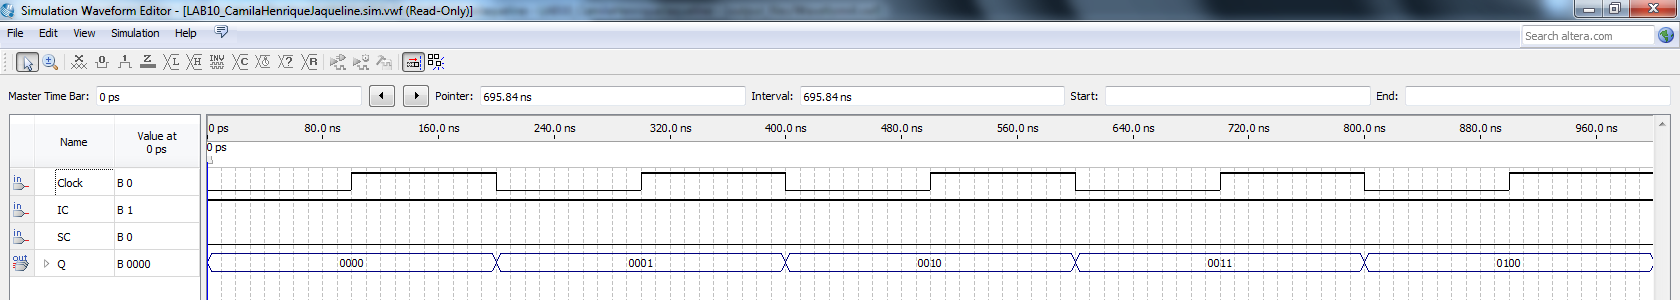
\includegraphics[width=1\textwidth]{contadorreversivelonda2.png}
		\caption{ Onda obtida quando a entrada IC se encontrava em 1 e a entrada SCse encontrava em 0 }
		\label{fig:contadorreversivelonda2}
	\end{figure}
	
	Aqui, como foi estabelecido que  SC = 0 seria a contagem progressiva, temos que a onda representa os estador corretamente, somando 1 a cada pulso do Clock.  Obs.: para o diagrama de ondas dessa parte do experimento, a ordem do nome das entradas foi trocada apenas para que os valores não ficassem ao contrário no diagrama de ondas, tornando a análise mais clara. 
	
	
	\begin{figure}[H]
		\centering
		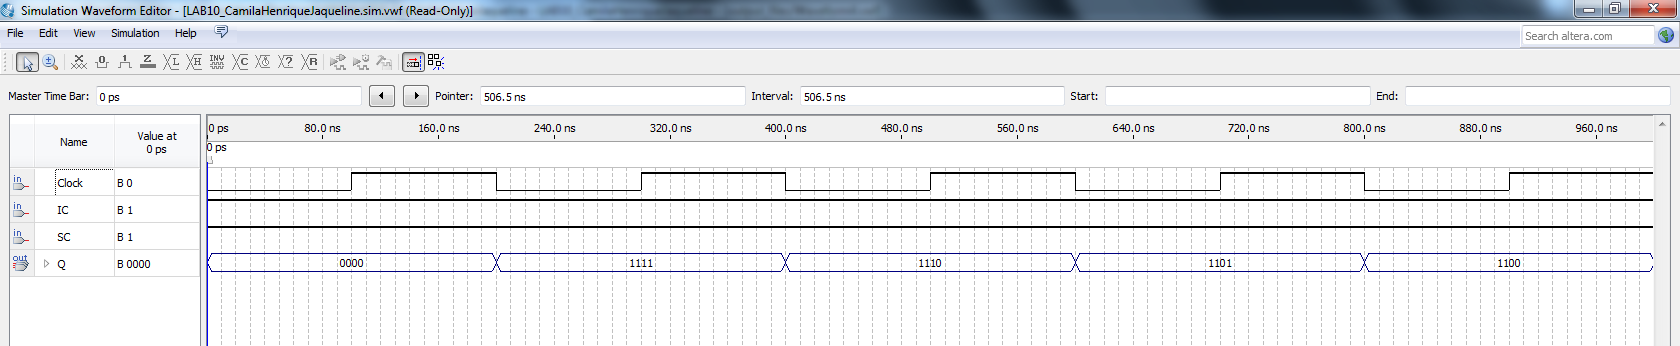
\includegraphics[width=1\textwidth]{contadorreversivelonda3.png}
		\caption{ Onda obtida quando a entrada IC se encontrava em 1 e a entrada SCse encontrava em 1 }
		\label{fig:contadorreversivelonda3}
	\end{figure}
	
	Vemos aqui que novamente o contador segue com o esperado decrementado o valor do último valor inserido. Além disso temos que o estado que segue o estado 0000 é 1111, mostrando que o laço contador funciona corretamente. As próximas figuras apenas detalham os resultados já apresentados:
	
	
	\begin{figure}[H]
		\centering
		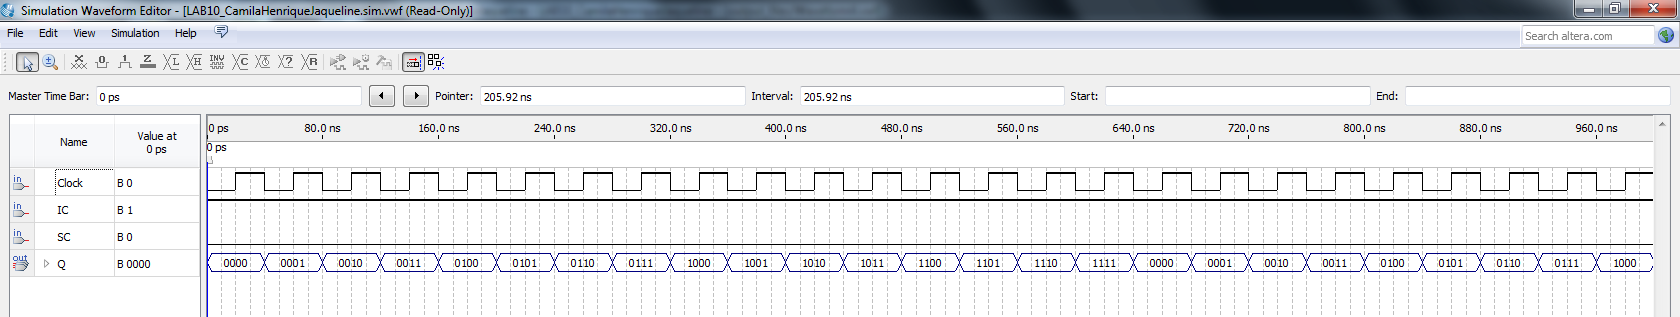
\includegraphics[width=1\textwidth]{contadorreversivelonda4.png}
		\caption{ Diagrama de ondas para SC = 0 }
		\label{fig:contadorreversivelonda4}
	\end{figure}
	
		\begin{figure}[H]
			\centering
			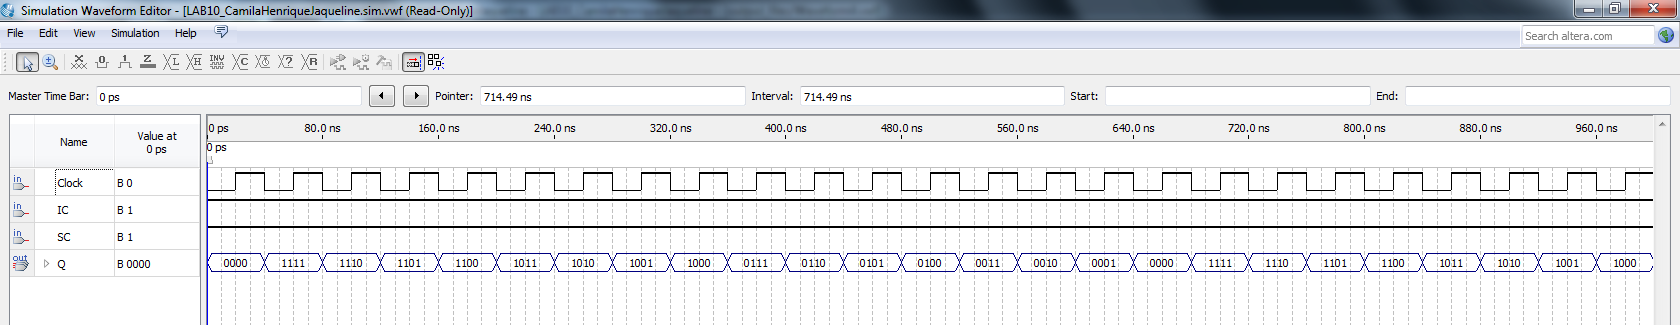
\includegraphics[width=1\textwidth]{contadorreversivelonda5.png}
			\caption{ Diagrama de ondas para SC = 1 }
			\label{fig:contadorreversivelonda5}
		\end{figure}



	
	\section{Conclusão}
	\label{sec:Conclusao}
	
	Neste experimento foi possível averiguar como atrasos de propagação podem afetar um circuito, gerando estados transitórios indesejados. Vemos que em circuitos sequenciais a prevenção desse tipo de atraso pode ser crucial dependendo do tipo de requisitos que o seu problema possui. Porém, também foi possível perceber que é possível tirar vantagem desses estados transitórios se analisarmos um circuito e soubermos quando e como esses estados ocorrerão. 

	\newpage 
	% Colocar aqui apenas as respostas dos itens da Auto-Avaliação
	\section*{Auto-Avaliação}
	
	\begin{enumerate}
		\item V
		\item V
		\item V
		\item V
		\item F
		\item V
		\item F
		\item V
		\item F
		\item V
		\item V
		\item F
		\item V
		\item V
		\item F
		\item F
		
	\end{enumerate}
	
	
\end{document}